% SRL research-article draft. SSA has no official LaTeX class; this follows the
% submission requirements (double-spaced, line-numbered, author-year citations,
% figures/tables with captions). Compile: tectonic manuscript.tex
\documentclass[12pt,letterpaper]{article}
\usepackage[margin=1in]{geometry}
\usepackage{amsmath,amssymb}
\usepackage{graphicx}
\usepackage{booktabs}
\usepackage{array}
\usepackage{longtable}
\usepackage{setspace}
\usepackage{lineno}
\usepackage[authoryear,round]{natbib}
\usepackage{xcolor}
\usepackage[font=small,labelfont=bf]{caption}
\usepackage{hyperref}
\hypersetup{colorlinks=true,linkcolor=black,citecolor=black,urlcolor=blue!60!black}
\graphicspath{{figures/}}

\newcommand{\Mw}{M_{\mathrm{w}}}
\newcommand{\todo}[1]{\textcolor{red}{[TODO: #1]}}
\newcommand{\verify}[1]{\textcolor{orange!80!black}{[verify: #1]}}
\newcommand{\Mdot}{\dot{M}}

\doublespacing
\linenumbers

\title{Supervising a causal GNSS magnitude network on released seismic moment yields PGD-like monotone convergence without early over-estimation}
\author{\todo{authors, affiliations, ORCIDs, corresponding author}}
\date{Draft v0.1 --- 8 September 2026}

\begin{document}
\maketitle

\noindent\small\textit{Draft note.} All numbers are taken from the frozen replays documented in the analysis report\\
\centerline{\path{docs/results/phase39-causal-released-moment/README.md}}\\
on branch \texttt{phase39-causal-released-moment-results}. Red items need author input; orange items were written from memory and must be checked before submission.
\normalsize

\section*{Abstract}

Real-time magnitude estimates from high-rate GNSS are attractive for large earthquakes because displacement does not saturate, but learned models that are asked at every second for the \emph{final} magnitude tend to answer with the training-set mean before enough waveform has arrived, producing early over-estimates that are later revised downward --- the opposite of the monotone rise of peak-ground-displacement (PGD) scaling. We show that this behaviour is a consequence of the supervision target rather than of the network. Keeping a physics-informed causal network unchanged (a 1.0-million-parameter temporal-convolution/transformer encoder that predicts a non-negative source time function and is regularised by a double-couple far-field forward operator), we replace the prefix target ``final moment magnitude'' by the \emph{released moment} $B_i(h)=\int_0^{h-\tau_{P,i}}\Mdot(t)\,dt$, i.e.\ the moment that station $i$ can causally have observed by time $h$ given its P-wave arrival $\tau_{P,i}$, and present prefixes by zero-padding so that the absolute source-time axis is preserved. On a fixed, event-disjoint split of 39 earthquakes ($\Mw$ 5.97--9.1, 2,694 station records), the change removes early over-estimation on every validation and test event within the training magnitude range (0 of 13 events above catalog magnitude at 1~s, versus 6 of 13 for the final-magnitude target), turns the event-median magnitude curve into a monotone approach from below that tracks the released moment of the SCARDEC source time function, and leaves 200-s endpoint accuracy and stabilisation time statistically indistinguishable from both the final-magnitude network and \citet{Crowell2013} PGD scaling on a single, pre-registered evaluation of seven held-out earthquakes within the training magnitude range (event MAE 0.18, 0.16 and 0.15 $\Mw$; median stable entry into $\pm0.3$ at 50, 56 and 52~s). The released-moment curve is a physical quantity at every second, not a forecast, and its residual against the label is a direct diagnostic: it exposes a learned distance prior --- far-field records in the training set come almost exclusively from $M\geq7.9$ Japanese events --- that over-estimates a dense-network $\Mw$~7.5 earthquake (Noto 2024) by 0.4 units while leaving an $\Mw$~8.2 event with the same network geometry (Tokachi 2003) unaffected. Two test earthquakes below the training minimum ($\Mw$ 6.0 and 6.2) are over-estimated by 0.7--1.4 units by every learned model, which fixes the method's operating range at $\Mw\geq6.4$ with the present data.

\section{Introduction}

Peak ground displacement (PGD) from high-rate GNSS scales with moment magnitude without the saturation that limits strong-motion amplitude measures for $M\gtrsim7$ \citep{Crowell2013,Melgar2015,Ruhl2019}. Because PGD is a running maximum of a causal quantity, the resulting magnitude estimate rises monotonically as the rupture unfolds and converges from below, a behaviour that operational systems value: an estimate that only grows never has to be retracted.

Learning-based alternatives have been proposed that map GNSS displacement records directly to magnitude \citep[e.g.][\verify{}]{Lin2021}, and physics-informed variants predict a source time function (STF) whose integral is the moment and whose forward-modelled displacement must match the observation. When such networks are trained \emph{causally} --- shown only the first $h$ seconds of each record and asked for the final magnitude at every $h$ --- they exhibit a failure mode that PGD does not: with little waveform available the loss-minimising answer is the conditional mean of the training set, so the 1-s estimate sits near $\Mw$~7.4 for every earthquake and is revised downward for small events and upward for great ones. In our earlier fixed-split experiment (the FINAL model of Section~\ref{sec:data}) this produced an early over-estimate on 3 of 6 validation and 5 of 9 test earthquakes.

We argue that this is not a property of the network but of the question it is asked. At time $h$ a station at hypocentral distance $r$ has recorded only the part of the rupture that radiated before $h-\tau_P(r)$; asking it for the \emph{final} moment is asking for a forecast, and a forecast under uncertainty regresses to the mean. Asking instead for the \emph{released} moment up to $h-\tau_P$ is asking for a quantity the data determine. The corresponding label is available from any published STF, and the target grows monotonically by construction.

This paper makes one change to a previously frozen causal model --- the prefix supervision target --- and evaluates it under a pre-registered protocol on a fixed event-disjoint split. We show that (i) the released-moment target removes early over-estimation and yields PGD-like monotone convergence; (ii) endpoint accuracy and stabilisation time are unchanged within the resolution of the test set; (iii) the released-moment residual is a diagnostic that isolates a data-coverage bias (a learned distance--magnitude prior) that a final-magnitude target hides; and (iv) the method's operating range is bounded below by the training magnitude range, and the early \emph{ranking} of events that the final-magnitude target obtains from its mean guess is not retained. We report negative results with the same weight as positive ones, including two knob experiments that did not remove the distance prior and a seed replicate that bounds the resolution of the validation set.

\section{Data}\label{sec:data}

\subsection{Events, records and split}

The dataset comprises 39 earthquakes with $\Mw$ 5.97--9.1 (2003--2024) recorded by high-rate GNSS at 1~Hz (Figure~\ref{fig:dataset}; Table~S1). For each station we use the radial (source-to-station) horizontal displacement over 200~s from the catalog origin time, baseline-corrected by the median of the 60~s preceding origin (falling back to the pre-P window when pre-origin data are missing), low-pass filtered at 0.2~Hz (7-tap Hamming FIR), and retained only if the record is $\geq99\%$ complete and its peak radial displacement exceeds 2~cm. This leaves 2,694 station records. \todo{GNSS data providers and processing (GEONET, EarthScope/UNAVCO, NGL, \ldots); positioning method; who computed the displacements}

Events were split \emph{by event} into 24 training (1,798 records), 6 validation (446) and 9 test (450) earthquakes before any model of this study was trained (split hash \texttt{e4807aa1\ldots}; Figure~\ref{fig:dataset}b--c). The split is not stratified by faulting style: training contains 16 reverse, 7 strike-slip and 1 normal event (84\% of records from reverse events, 66\% from Tohoku 2011 and Ibaraki 2011 alone); validation contains 2/3/1 and test 4/3/2. The smallest training event is $\Mw$~6.4; validation includes one and test two events below that limit (Parkfield 2004, 5.97; Napa 2014, 6.02; ak014cbigci8, 6.20).

\subsection{Source time functions}

Labels are SCARDEC moment-rate functions \citep{Vallee2011,Vallee2016}, resampled to 1~s over 0--200~s from origin and rescaled so that their integral equals the catalog moment (GCMT/USGS $\Mw$). The rescaling keeps SCARDEC's shape and removes its absolute-moment offset (e.g.\ 8.79 versus 8.80 for Maule 2010), so that ``released moment'' and ``catalog magnitude'' refer to the same scale.

\subsection{Baselines}

We compare against three PGD scaling laws evaluated on the same stations with the same causal prefixes --- \citet{Crowell2013}, \citet{Melgar2015} and \citet{Ruhl2019} --- each as an event median of station estimates at every second, PGD being the running maximum of the three-component displacement up to $h$ \verify{component convention of the PGD baseline code}. We note that these laws are not held out: \citet{Crowell2013} were fit on Tokachi-oki 2003 (43 stations), El Mayor--Cucapah 2010, Tohoku-oki 2011 and two 2012 Brawley events, and \citet{Melgar2015} on a set that includes Iquique 2014 and Napa 2014 (our test set) and Maule 2010 and Parkfield 2004 (our validation set). The comparison therefore favours the scaling laws.

We also compare against the \emph{same network trained with the final-magnitude prefix target} (hereafter FINAL; checkpoint \texttt{4a254024\ldots}), which had been selected and evaluated once on the test set in the preceding study.

\section{Method}

\subsection{Network and physics (unchanged)}

The network (Figure~\ref{fig:method}a) takes the radial displacement record and four geometric inputs ($\ln r$, $\sin\theta$, $\cos\theta$, $\sin\varphi$, $\cos\varphi$ for hypocentral distance $r$, take-off angle $\theta$ and azimuth $\varphi$) and outputs a non-negative moment-rate function $\Mdot(t)=M_0\,p(t)$ on 200 one-second bins, factorised into a scalar moment $M_0$ and a normalised shape $p(t)$. The encoder is a six-block temporal convolutional network \citep{Bai2018} followed by a three-layer transformer \citep{Vaswani2017} (hidden width 128, dropout 0.2; 1,010,850 trainable parameters). A double-couple far-field forward operator ($\rho=3400$~kg\,m$^{-3}$, $\alpha=7.9$~km\,s$^{-1}$, $\beta=4.53$~km\,s$^{-1}$, P and S terms, absolute travel-time delays) maps $\Mdot$ and the station geometry to a synthetic radial displacement $\hat u(t)$, and an amplitude-normalised, polarity-tolerant misfit $\mathcal{L}_\mathrm{synth}$ between $\hat u$ and the observed $u$ regularises the STF (weight $\lambda_\mathrm{synth}=0.5$). The endpoint loss on the full 200-s window is the mean-squared error on $\log_{10}(1+\Mdot/10^{18})$ plus a magnitude term. All of this is inherited from the frozen FINAL model and was not tuned in this study.

\subsection{Causal prefixes}

Training and evaluation are causal: the network sees only samples $t<h$ of the displacement record. Each optimisation step processes the full 200-s window and two prefixes $h$ and $h+10$~s with $h$ drawn uniformly from $[5,189]$~s (the pair is retained from the FINAL recipe and is inert here, see below). We changed how a prefix is \emph{presented}: FINAL truncated the record to $h$ samples and stretched it to the 200-step input length, which discards the absolute time axis; we instead zero-pad the truncated record to 200~s, so that source time and observation time share one origin and $\tau_P$ has a meaning inside the network.

\subsection{Released-moment target}

For station $i$ with P arrival $\tau_{P,i}=r_i/\alpha$ and prefix $h$, the constrained source window is $[0,\,h-\tau_{P,i}]$. The released moment and magnitude are
\begin{equation}
M^{\mathrm{rel}}_i(h)=\sum_{k} m_{ik}(h)\,\max(\Mdot_{ik},0)\,\Delta t,\qquad
m_{ik}(h)=\mathrm{clip}\!\left(\frac{h-\tau_{P,i}}{\Delta t}-k,\;0,\;1\right),
\end{equation}
\begin{equation}
B_i(h)=\tfrac{2}{3}\left(\log_{10}\max\!\left(M^{\mathrm{rel}}_i(h),10^{15}\right)-9.1\right),
\end{equation}
with the same operator applied to the SCARDEC label to give the target $B^{\mathrm{ref}}_i(h)$ (Figure~\ref{fig:method}b--c). The floor $10^{15}$~N\,m ($\Mw$~3.93) makes $B$ well defined before P arrival. The prefix losses are the STF mean-squared error restricted to the constrained window and $|B_i-B^{\mathrm{ref}}_i|$; prefixes with $h-\tau_{P,i}<1$~s contribute only $\mathcal{L}_\mathrm{synth}$. The FINAL model's ``error-descent'' term, which compared the prefix's final-magnitude estimate to the endpoint, has no analogue and is removed. The final magnitude $A_i(h)$, obtained by integrating the \emph{whole} predicted STF, is still available at every prefix and is reported alongside $B$.

Two reporting conventions follow from causality. The event curve $B^*(h)$ is the median of $B_i(h)$ over stations whose window is at least 1~s (P has arrived), mirroring PGD's ``wherever defined''; $A(h)$ is the median over all stations. At $h=200$~s, $B^*=A$ for every station in our data.

\subsection{Counterfactual moment scaling}

The training set contains no event below $\Mw$~6.4. Following the FINAL recipe, each training record is augmented by a counterfactual copy in which waveform, label STF and target moment are multiplied by $10^{1.5\,\Delta\Mw}$ with $\Delta\Mw$ uniform on an interval; FINAL used $[-0.75,\,0.5]$. We widened the lower bound to $-1.0$ (variant NEW-3 below) so that synthetic $\Mw$ 5.4--5.9 examples exist. This is the only hyper-parameter changed from FINAL.

\subsection{Training and protocol}

AdamW \citep{Loshchilov2019} (learning rate $10^{-4}$, weight decay $10^{-5}$), cosine schedule with 5 warm-up epochs, batch 64, up to 200 epochs with early stopping (patience 50) on the fixed validation set, event-balanced inverse-count sample weights, seed 73. Before training we pre-registered five validation gates (Table~\ref{tab:validation}) and the rule ``two knobs, then stop'': the released-moment target (NEW-1), a monotone pair penalty $\mathrm{ReLU}\!\left(B(h)-B(h+10)-0.03\right)^2$ (NEW-2, weight 0.5) and the wider scaling interval (NEW-3). Model selection used only the six validation events. The test set was not loaded by any training run (every run manifest records \mbox{\texttt{held\_out\_test\_loader\_iterated}} \texttt{= false}) and was evaluated once, on 8 September 2026, after NEW-3 had been declared the final candidate; no model was modified afterwards.

\subsection{Objective metrics}

At every second we report the event-median magnitude curve and, per event: the 200-s error against catalog $\Mw$; whether the 1-s estimate exceeds catalog; the number of sign changes of the first difference of $B^*$ (jitter); the \emph{stable-entry time}, the earliest second after which the curve never leaves $\pm0.3$ of catalog; and Spearman rank correlation with catalog $\Mw$ across events at fixed $h$.

\section{Results}

\subsection{Validation (6 events, 446 records)}

\paragraph{Curve shape.} Figure~\ref{fig:valtraj} shows the event curves. FINAL (grey) starts near $\Mw$~7.4 on every event and descends; three of six events are above catalog at 1~s. NEW-3 (red) starts at the floor before P arrival, rises after it, and converges from below onto the released moment of the SCARDEC label (green dotted): the 1-s final-magnitude prior falls from 7.44 to 6.32 and no event is above catalog at 1~s (Table~\ref{tab:validation}). The three released-moment variants are nearly indistinguishable in shape; they differ on Parkfield, where widening the scaling interval removes a $+0.2$ over-estimate, and in the size of the Noto over-estimate.

\paragraph{Endpoint.} At 200~s the event MAE is 0.090 for NEW-3, 0.127 for FINAL and 0.169 for Crowell PGD (0.337 Melgar, 0.522 Ruhl; Figure~\ref{fig:valend}, Table~\ref{tab:validation}); five of six events are within $\pm0.09$. Training-set MAE moves the other way (0.109 versus 0.092 for FINAL): the released-moment target fits the training events less tightly and generalises better on this split. A second seed (42) of the NEW-3 recipe gives 0.105, so the seed-to-seed spread is $\approx0.015$~$\Mw$; differences smaller than this between variants are not interpreted.

\paragraph{Stabilisation.} $B^*$ enters $\pm0.3$ permanently on five of six events (median 60~s; FINAL 65~s; Crowell 87~s) and does so before Crowell on four (Parkfield 7 versus 8~s, Anchorage 20 versus 33~s, SandPoint 60 versus 99~s, Rat Islands 117~s versus never), the same count as FINAL. Maule ($\Mw$~8.8) is the exception: $B^*$ drops from 8.3 to 7.35 near 65--70~s and then climbs with Crowell, entering at 181~s; the SCARDEC label itself needs 116~s.

\paragraph{Jitter.} The mean number of sign changes over 200~s is 29.5 for NEW-3 and 41 for FINAL, both far above the pre-registered threshold of 10; the monotone pair penalty (NEW-2) did not reduce it (33.7). Every second is an independent forward pass with no state carried between prefixes, so adjacent estimates are not constrained to be consistent. A causal post-filter (5-s exponential average followed by an envelope allowing at most 0.005~$\Mw$\,s$^{-1}$ decrease) brings sign changes to 8.3 at the cost of a $\approx5$~s lag that raises the 200-s MAE to 0.100 and moves Parkfield's stable entry from 7 to 12~s; scanning the averaging constant from 2 to 12~s shows a strict jitter--lag trade-off (Figure~S3 \todo{promote report Figure 12 if kept}).

\paragraph{Gates.} NEW-3 passes three of five pre-registered gates (endpoint MAE below both FINAL and Crowell, no 1-s over-estimate, earlier-than-Crowell on $\geq4/6$) and fails two (jitter; rank correlation of $B^*$ at 30~s $\geq0.94$). The second failure is a mis-specified gate: at 30~s $B^*$ is a released moment, so Maule correctly ranks below Noto, and rank correlation with \emph{final} magnitude penalises the physically right answer. The same network's $A(30~\mathrm{s})$ ranks the six events with $\rho=0.94$, equal to FINAL. Because the gates were not all passed, the pre-registered rule required stopping; the test evaluation below is a deliberate, recorded termination of that protocol, not a pass.

\subsection{How close is the predicted STF to the label?}

The released-moment target constrains the \emph{integral} of $\Mdot$ inside the constrained window, not its shape. Comparing predicted and label STFs station by station (Figure~\ref{fig:method}b for one station; report Figure~4C--D for all 446), the event-median shape correlation inside the window rises from $\approx0.5$ at 30--90~s to 0.73 at 200~s (FINAL 0.76), while the event-level error of the released magnitude inside the window is already 0.16--0.27 at 30--90~s and 0.09 at 200~s. The model learns \emph{how much} has been released before it learns \emph{when}. For the station shown in Figure~\ref{fig:method}, the 200-s shape correlation is 0.89 and the released-magnitude error $-0.08$.

\subsection{Why Noto 2024 is over-estimated}

Noto ($\Mw$~7.5, 397 stations, 89\% of validation records) is over-estimated by $+0.39$ (NEW-3) and $+0.34$ (FINAL) at 200~s. Three hypotheses were tested (report Figure~13). The label is not the cause (SCARDEC 7.51 versus catalog 7.50). Near-field saturation is not the cause: the three stations within 50~km have a median error of $-0.19$, whereas the 394 stations at 50--500~km are uniformly $+0.31$ to $+0.44$. The cause is a learned geometry prior: the network's final-magnitude estimate \emph{before any signal has arrived}, $A(1~\mathrm{s})$, is almost a deterministic function of hypocentral distance (correlation 0.96 with $\ln r$ across all training and validation records, versus 0.65 with catalog magnitude). Of the 1,183 training records beyond 200~km, 53\% belong to Tohoku 2011 ($\Mw$~9.1) and 28\% to Ibaraki 2011 ($\Mw$~7.9): in the training distribution, ``a far-field record that passed the 2-cm quality threshold'' implies an $M\geq7.9$ Japanese earthquake. Noto has 278 stations beyond 200~km on the same network. The prior is visible only because the released-moment residual is a physical quantity; a final-magnitude network absorbs it into its early guess.

Two knobs aimed at the prior were tried after the pre-registered protocol had ended and are reported as negative results: replacing inverse-count event weights by event-balanced resampling (Noto $+0.37$; no change within seed noise) and sampling more negative $\Delta\Mw$ for far stations (100--300~km transition to $[-1.5,0]$; Noto $+0.31$ but Anchorage and SandPoint pushed to $-0.12$ and $-0.09$). Weighting cannot create the missing cell --- moderate-magnitude far-field records --- in the training distribution.

\subsection{Held-out test (evaluated once)}

Table~\ref{tab:test} and Figures~\ref{fig:testend}--\ref{fig:testtraj} give the single test evaluation. Two of the nine events (Napa 2014, $\Mw$~6.02; ak014cbigci8, 6.20) lie below the training minimum of 6.4 and are over-estimated by every learned model (NEW-3 $+0.68$ and $+1.35$; FINAL $+0.67$ and $+1.27$; the non-causal endpoint model of the preceding study $+0.84$ and $+0.99$); Crowell PGD over-estimates them by $+0.90$ and $+0.86$. We therefore state the operating range of the method as $\Mw\geq6.4$ with the present training data and report the seven in-range events (418 records) as the primary result, keeping all nine in Table~\ref{tab:test}. The criterion is the training range, fixed before testing; the worst in-range event is retained.

Within range, the 200-s event MAE is 0.180 for NEW-3, 0.160 for FINAL and 0.149 for Crowell (RMSE 0.225, 0.185, 0.183); six of seven events are within $\pm0.3$ for all three. Per event, NEW-3 beats Crowell on Puebla, Ecuador and Iquique, ties (within 0.02) on Ridgecrest and Tokachi, and loses on 2016p661332 ($+0.45$ versus $+0.05$; 7 stations, normal faulting, New Zealand) and us7000i9bw ($-0.28$ versus $+0.10$). The whole MAE difference to Crowell is carried by 2016p661332. With seven events, differences of 0.03 are not resolvable, and the validation-set advantage of NEW-3 over FINAL (0.090 versus 0.127) did not carry over; we conclude that endpoint accuracy is unchanged by the target, not improved.

The curve-shape result does carry over. No in-range event is above catalog at 1~s (FINAL: 3 of 7); over all nine the count is 1 versus 5, the exception being ak014cbigci8 ($\Mw$~6.20), which the 1-s prior of 6.35 exceeds by 0.15. The mean 1-s final-magnitude prior is 6.23 versus 7.47, and $B^*$ approaches from below on every event (Figure~\ref{fig:testtraj}). Stable entry into $\pm0.3$ occurs on six of seven events with a median of 50~s (FINAL 56.5~s, Crowell 52~s); NEW-3 is earlier than Crowell on Puebla (21 versus 42~s), us7000i9bw (48 versus 62~s) and Ecuador (52 versus 88~s), equal on Ridgecrest (26~s), one second later on Tokachi (96 versus 95~s), enters on Iquique at 87~s where Crowell never does, and never enters on 2016p661332 where Crowell does at 10~s. Jitter is unchanged (40 sign changes per event in range; FINAL 41).

One validation-stage result did not carry over. At 30~s the rank correlation of the final-magnitude estimate $A$ with catalog $\Mw$ across the nine test events is 0.19 for NEW-3 against 0.89 for FINAL (60~s: 0.85 versus 0.96); $B^*$ and Crowell PGD also give 0.19 at 30~s. FINAL's early ranking rests on the same conditional-mean guess that produces its early over-estimation --- it places every event near 7.5 at 1~s and then moves each in the right direction --- and the released-moment target, which forbids the guess, does not retain that ordering. Whether early \emph{ranking} or early \emph{non-over-estimation} matters more is an operational choice; we report both.

Tokachi-oki 2003 ($\Mw$~8.16, 228 stations, mostly far-field, same GEONET geometry as Noto) is estimated at 8.10 ($-0.06$). The distance prior that over-estimates Noto therefore harms only events whose true magnitude is \emph{below} what the far-field geometry implies; for an $M\approx8$ earthquake prior and truth agree.

\section{Discussion}

\paragraph{What the target changes and what it does not.} The released-moment target is a statement about what a station can know at time $h$. Supervising on it removes the incentive to guess: before P arrival the correct answer is the floor, and after it the correct answer grows with the rupture. The observed consequences --- no early over-estimation, monotone approach from below, agreement with the released moment of the label --- follow directly, and they hold on every validation and test event including those outside the training range. What the target does \emph{not} change is the information content of the waveform at 200~s: endpoint accuracy is the same as with the final-magnitude target and the same as PGD scaling, within the resolution of 6--7 events. We consider this the honest reading of Tables~\ref{tab:validation}--\ref{tab:test} and recommend against reading the validation-set improvement as a gain.

\paragraph{A physical intermediate quantity as a diagnostic.} Because $B(h)$ is a released moment, its residual against $B^{\mathrm{ref}}(h)$ can be interpreted. The Noto analysis illustrates the value: the same over-estimate is present in FINAL, but there it is indistinguishable from an early guess, whereas in NEW-3 it appears after 60~s, when the rupture has ended, as moment being added to the STF in the constrained window --- a learned prior, localised to far stations, traceable to two training events. The remedy is data (moderate-magnitude events with far-field coverage, or distance-aware post-calibration), not architecture or loss weights, and the two failed knob experiments confirm this.

\paragraph{Jitter is structural.} Each second is an independent inference; nothing ties $B(h)$ to $B(h-1)$. A causal filter trades jitter for lag one-for-one. A stateful moment head, or supervising on increments $B(h)-B(h-1)\geq0$ with a recurrent state, is the natural next step and was outside the scope of this single-change study.

\paragraph{Comparison with PGD scaling.} PGD reaches its final value when the peak displacement has passed every station; the released-moment network reaches it when the constrained window covers the STF, which is earlier for stations near the source. On the test set this produced earlier stabilisation on three of the five events where both converge, and a stable estimate on Iquique, where the PGD law never converged to within 0.3; the reverse happened on 2016p661332, where the network's $+0.45$ endpoint never entered the band. Against this, the network jitters and PGD does not, and the network's operating range is bounded by its training data while a scaling law extrapolates smoothly (Crowell's errors on the two small events, $+0.9$, are smaller than the network's $+1.35$). We also note again that the scaling laws were fit on data that include four of our fifteen validation/test earthquakes.

\paragraph{Faulting style.} The training set is dominated by reverse faulting, but 200-s errors do not separate by mechanism on training or validation events (Figure~S1), and the single normal-faulting validation event (Anchorage, 47~km deep) and the intermediate-depth Rat Islands event (109~km, 60~km deeper than any training event) are within $\pm0.08$. The one in-range test failure (2016p661332) is a normal-faulting event with seven stations; with one sample we cannot separate mechanism from station count.

\section{Limitations}

\begin{enumerate}
\item \textbf{Operating range.} No training event below $\Mw$~6.4; the two test events below it are over-estimated by 0.7--1.4~$\Mw$ by every learned model. Counterfactual down-scaling to $\Delta\Mw=-1$ does not substitute for real small-event network geometry.
\item \textbf{Sample size.} Six validation and seven in-range test events; seed-to-seed spread 0.015~$\Mw$; a single event (2016p661332, $+0.45$) decides the ranking against PGD.
\item \textbf{Distance prior.} Far-field training records come almost exclusively from two $M\geq7.9$ events; dense-network $M$~7--7.5 earthquakes are over-estimated (Noto $+0.39$).
\item \textbf{Jitter.} $\approx$30--40 sign changes per 200~s; removable only by a filter that adds $\approx5$~s of lag.
\item \textbf{Early ranking.} At 30~s the released-moment model ranks the test events no better than PGD ($\rho=0.19$), whereas the final-magnitude model's early guess ranks them at 0.89; the two targets trade early ranking against early over-estimation.
\item \textbf{Single fold, single architecture.} One fixed split; the physics operator, network and endpoint loss were inherited unchanged and not re-optimised for the new target.
\item \textbf{Label dependence.} Released-moment labels require a published STF; SCARDEC coverage limits the event set and its shapes are themselves inversions with uncertainty we do not propagate.
\end{enumerate}

\section{Conclusions}

Changing the prefix supervision target of a causal GNSS magnitude network from final magnitude to released moment --- with no change to the network, the physics operator or the endpoint loss --- removes early over-estimation and produces PGD-like monotone convergence on every validation and held-out test earthquake, at endpoint accuracy and stabilisation time that are indistinguishable from the original network and from PGD scaling within the resolution of the data. The released-moment curve is a physical quantity at every second and its residual is a usable diagnostic; it exposed a distance--magnitude prior inherited from the training set's far-field coverage. With the present data the method operates for $\Mw\geq6.4$. Second-to-second jitter remains and requires a stateful formulation.

\section*{Data and Resources}

GNSS displacement records: \todo{providers, access dates, processing centre}. SCARDEC source time functions: \url{http://scardec.projects.sismo.ipgp.fr} \citep{Vallee2016}, accessed \todo{date}. Catalog magnitudes: Global CMT (\url{https://www.globalcmt.org}) and USGS ComCat. Code, configuration files, frozen checkpoint hashes, per-second predictions and the full analysis report are available at \todo{Zenodo DOI}; the development record is in the repository branch \texttt{phase39-causal-released-moment-results}. All figures are generated from frozen inference replays by \path{scripts/plotting/plot_srl_released_moment_figures.py}.

\section*{Declaration of Competing Interests}

The authors declare no competing interests.

\section*{Acknowledgments}

\todo{acknowledgments}

\bibliographystyle{plainnat}
\bibliography{references}

\clearpage
\section*{Tables}

\begin{table}[h]
\centering
\caption{Validation objective metrics and pre-registered gates (6 events, 446 records). FINAL: final-magnitude prefix target; NEW-1: released-moment target; NEW-2: NEW-1 + monotone pair penalty; NEW-3: NEW-1 + scaling interval $[-1.0,0.5]$ (final candidate). Bold marks the pre-registered gates NEW-3 passes.}
\label{tab:validation}
\resizebox{\textwidth}{!}{%
\begin{tabular}{lrrrrr}
\toprule
 & FINAL & NEW-1 & NEW-2 & NEW-3 & Crowell \\
\midrule
200-s event MAE & 0.127 & 0.118 & 0.122 & \textbf{0.090} & 0.169 \\
Events above catalog at 1~s ($A$) & 3 & 1 & 1 & \textbf{0} & 0 \\
Mean sign changes of $B^*$ & 41.0 & 29.8 & 33.7 & 29.5 & 0 \\
Stable entry $\pm0.3$: events / median & 5 / 65~s & 6 / 70.5~s & 5 / 73~s & 5 / 60~s & 5 / 87~s \\
Earlier than Crowell & 4/6 & 3/6 & 3/6 & \textbf{4/6} & --- \\
Spearman $\rho$ at 30~s, $B^*$ / $A$ & 0.71 / 0.94 & 0.77 / 0.77 & 0.89 / 0.94 & 0.77 / 0.94 & 0.83 \\
\bottomrule
\end{tabular}}
\end{table}

\begin{table}[h]
\centering
\caption{Held-out test, single evaluation. Primary rows: the seven events within the operating range $\Mw\geq6.4$ (418 records). Lower rows: all nine events and the two below-range events.}
\label{tab:test}
\resizebox{\textwidth}{!}{%
\begin{tabular}{lrrrrr}
\toprule
$\Mw\geq6.4$, 7 events & NEW-3 & FINAL & Crowell & Melgar & Ruhl \\
\midrule
200-s event MAE / RMSE & 0.180 / 0.225 & 0.160 / 0.185 & \textbf{0.149 / 0.183} & 0.290 / 0.336 & 0.469 / 0.502 \\
Events within $\pm0.3$ & 6/7 & 6/7 & 6/7 & 4/7 & 2/7 \\
Per event vs Crowell: win / tie / loss & 3 / 2 / 2 & 3 / 1 / 3 & --- & --- & --- \\
Above catalog at 1~s ($A$; 1-s mean) & \textbf{0} (6.23) & 3 (7.47) & 0 & 0 & 0 \\
Stable entry $\pm0.3$: events / median & 6 / 50~s & 6 / 56.5~s & 6 / 52~s & 4 / 94.5~s & 2 / 127.5~s \\
Mean sign changes of $B^*$ & 40.4 & 41.1 & 0 & 0 & 0 \\
\midrule
All 9: Spearman $\rho$ of $A$, 30~s / 60~s & 0.19 / 0.85 & 0.89 / 0.96 & 0.19 / 0.85 & $-0.15$ / 0.48 & $-0.15$ / 0.48 \\
All 9: 200-s MAE & 0.366 & 0.340 & 0.311 & 0.357 & 0.445 \\
All 9: above catalog at 1~s ($A$) & 1 & 5 & 0 & 0 & 0 \\
Napa 6.02 / ak014cbigci8 6.20: error & $+0.68$ / $+1.35$ & $+0.67$ / $+1.27$ & $+0.90$ / $+0.86$ & --- & --- \\
\bottomrule
\end{tabular}}
\end{table}

\clearpage
\section*{Figures}

\begin{figure}[p]
\centering
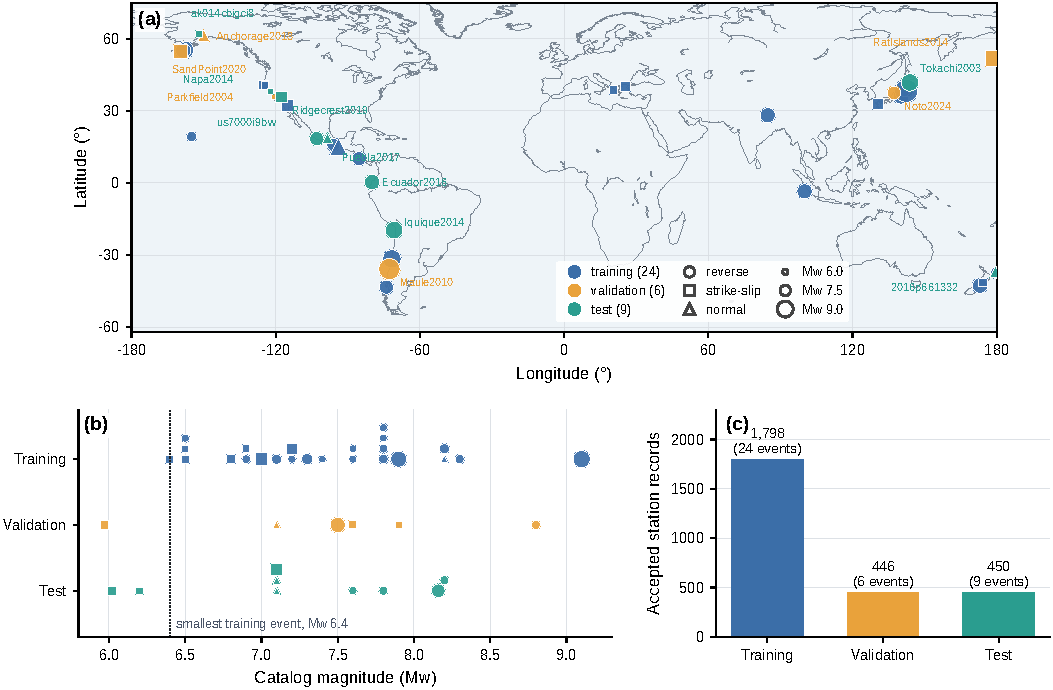
\includegraphics[width=\textwidth]{fig1_dataset.pdf}
\caption{Dataset. (a) Epicentres of the 39 earthquakes coloured by cohort (training 24, validation 6, test 9); marker shape gives faulting style, size gives $\Mw$. (b) Catalog magnitude by cohort; the dotted line is the smallest training event ($\Mw$~6.4). (c) Accepted station records per cohort.}
\label{fig:dataset}
\end{figure}

\begin{figure}[p]
\centering
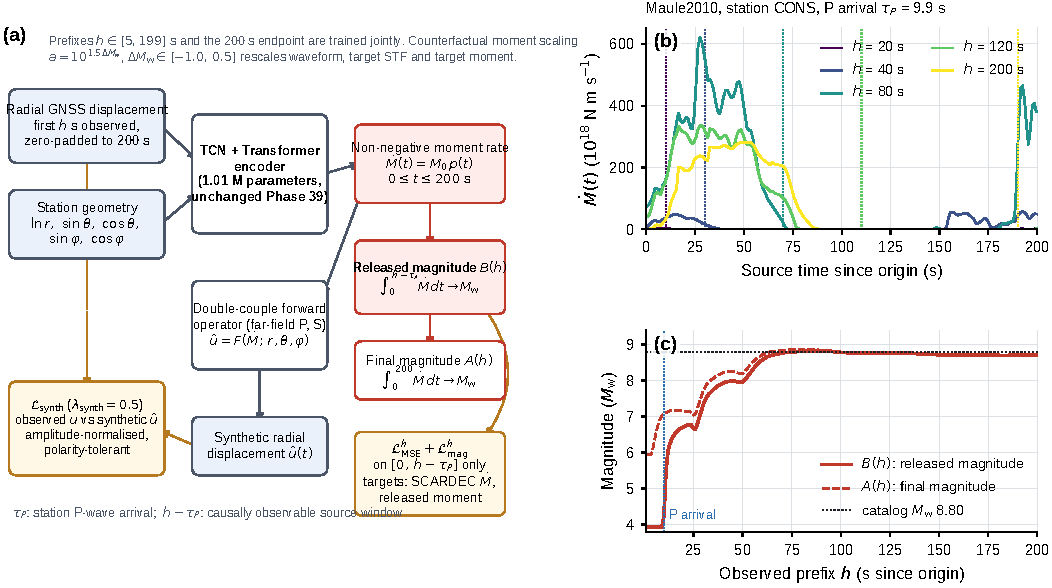
\includegraphics[width=\textwidth]{fig2_method.pdf}
\caption{Method. (a) Data flow. The radial GNSS record, zero-padded beyond the observed prefix $h$, and station geometry enter a TCN--transformer encoder that outputs a non-negative moment rate $\Mdot(t)$; a double-couple forward operator produces a synthetic displacement whose misfit ($\mathcal{L}_\mathrm{synth}$) regularises $\Mdot$. The prefix losses act only on the causally observable window $[0,h-\tau_P]$ and target the released moment of the SCARDEC label. (b) Predicted $\Mdot$ for Maule 2010 station CONS ($\tau_P=9.9$~s) at five prefixes; dotted verticals mark $h-\tau_P$. (c) Released magnitude $B(h)$ and final magnitude $A(h)$ for the same station.}
\label{fig:method}
\end{figure}

\begin{figure}[p]
\centering
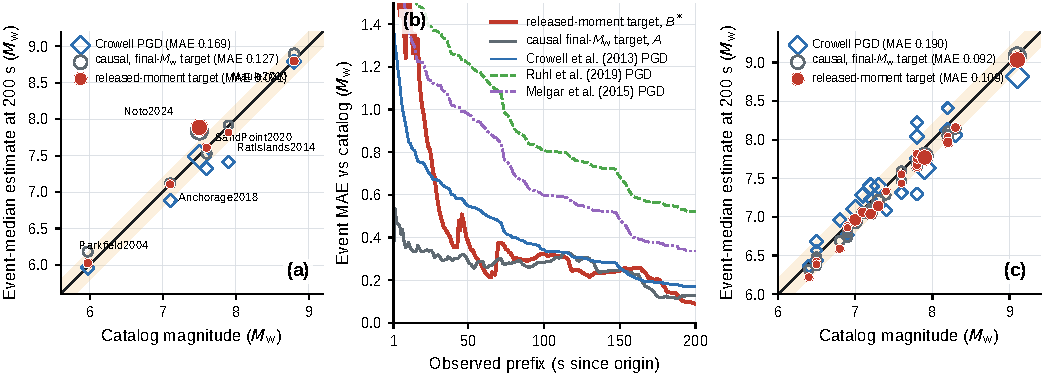
\includegraphics[width=\textwidth]{fig3_validation_endpoint.pdf}
\caption{Validation endpoint (6 events, 446 records). (a) Event-median estimate at 200~s versus catalog $\Mw$ for the released-moment model, the final-magnitude model and Crowell PGD; marker size scales with station count. (b) Event MAE versus observed prefix. (c) Absolute 200-s error per event.}
\label{fig:valend}
\end{figure}

\begin{figure}[p]
\centering
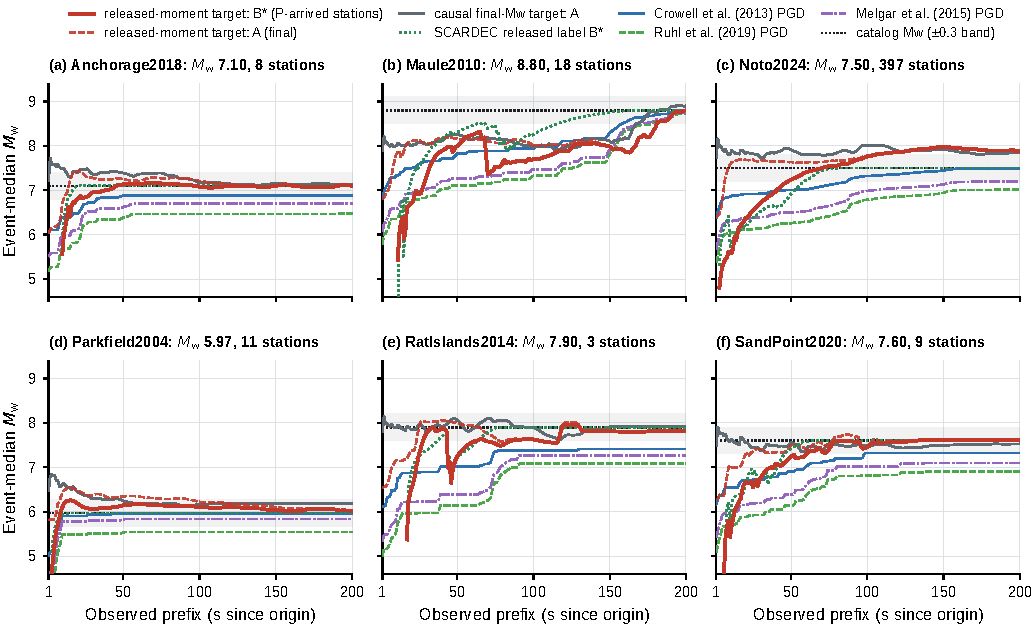
\includegraphics[width=\textwidth]{fig4_validation_trajectories.pdf}
\caption{Validation event curves. Released magnitude $B^*$ (solid red; P-arrived stations) and final magnitude $A$ (dashed red) of the released-moment model, $A$ of the final-magnitude model (grey), released magnitude of the SCARDEC label (green dotted), Crowell/Ruhl/Melgar PGD and catalog $\Mw$ with $\pm0.3$ band.}
\label{fig:valtraj}
\end{figure}

\begin{figure}[p]
\centering
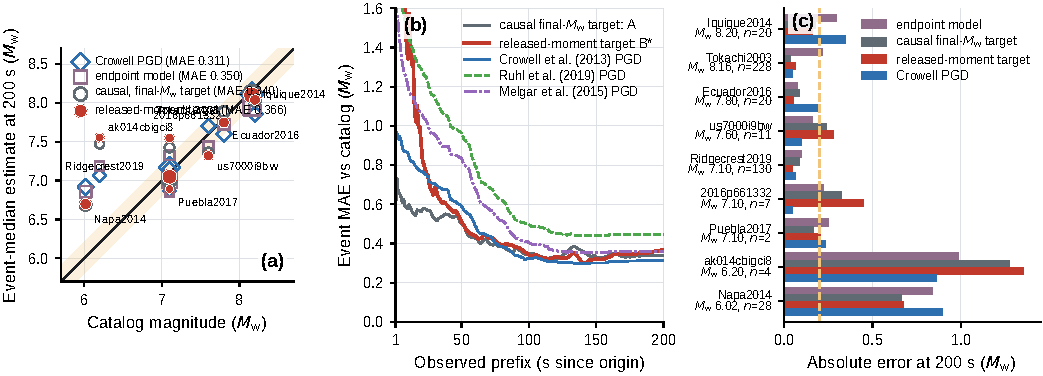
\includegraphics[width=\textwidth]{fig5_test_endpoint.pdf}
\caption{Held-out test (single evaluation; 9 events, 450 records). (a) 200-s estimates versus catalog; legend MAEs are over the seven events within the operating range $\Mw\geq6.4$ (shaded band marks the two below it). (b) Event MAE versus prefix. (c) Absolute 200-s error per event for the endpoint model of the preceding study, the final-magnitude causal model, the released-moment model and Crowell PGD.}
\label{fig:testend}
\end{figure}

\begin{figure}[p]
\centering
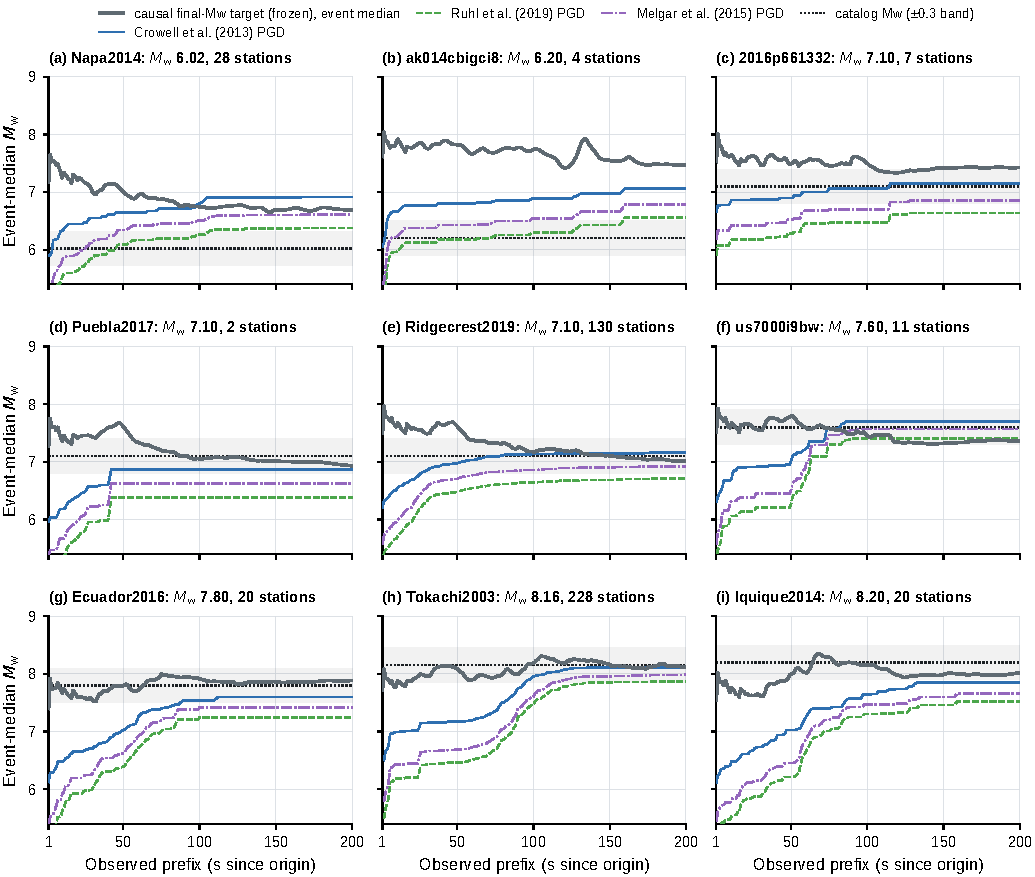
\includegraphics[width=\textwidth]{fig6_test_trajectories.pdf}
\caption{Test event curves, as Figure~\ref{fig:valtraj}. Napa 2014 and ak014cbigci8 are below the training minimum.}
\label{fig:testtraj}
\end{figure}

\clearpage
\section*{Supplementary Material}

\begin{figure}[p]
\centering
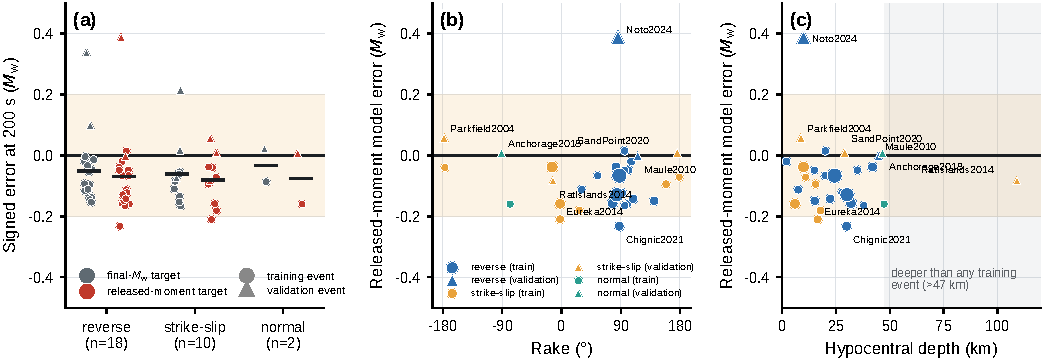
\includegraphics[width=\textwidth]{figS1_mechanism.pdf}
\caption*{\textbf{Figure S1.} Signed 200-s error by faulting style, rake and depth (training and validation).}
\end{figure}

\begin{figure}[p]
\centering
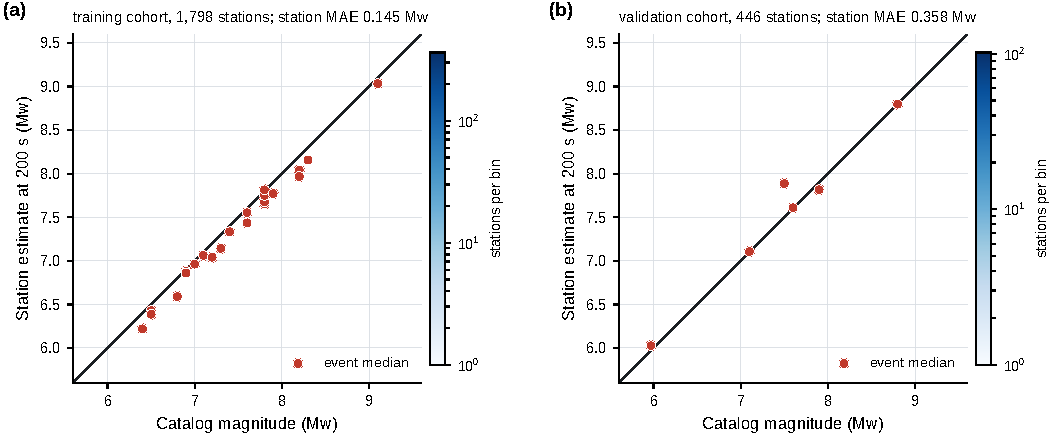
\includegraphics[width=\textwidth]{figS2_station_scatter.pdf}
\caption*{\textbf{Figure S2.} Station-level 200-s estimates (training and validation).}
\end{figure}

\clearpage
\singlespacing
\footnotesize
\setlength{\LTcapwidth}{\textwidth}
\begin{longtable}{@{}lccclrrrr@{}}
\caption*{\textbf{Table S1.} Events, cohorts, faulting style, depth, accepted stations and signed 200-s event error (estimate $-$ catalog) of the released-moment model (NEW-3), the final-magnitude model (FINAL) and Crowell PGD.}\\
\toprule
Event & Origin date & $M_{\mathrm{w}}$ & Mechanism & Depth (km) & Stations & NEW-3 & FINAL & Crowell \\
\midrule
\endfirsthead
\toprule
Event & Origin date & $M_{\mathrm{w}}$ & Mechanism & Depth (km) & Stations & NEW-3 & FINAL & Crowell \\
\midrule
\endhead
\bottomrule
\endfoot
\multicolumn{9}{@{}l}{\textit{Training cohort} (24 events, 1,798 records)} \\
nc73821036 & 2022-12-20 & 6.40 & strike-slip & 18 & 9 & -0.18 & -0.08 & -0.04 \\
2013p543824 & 2013-07-21 & 6.50 & strike-slip & 16 & 8 & -0.09 & -0.05 & -0.06 \\
2013p613797 & 2013-08-16 & 6.50 & reverse & 8 & 10 & -0.11 & -0.02 & +0.18 \\
Lefkada2015 & 2015-11-17 & 6.50 & strike-slip & 11 & 3 & -0.07 & -0.13 & +0.07 \\
Eureka2014 & 2014-03-10 & 6.80 & strike-slip & 17 & 15 & -0.21 & -0.11 & +0.16 \\
Aegean2014 & 2014-05-24 & 6.90 & strike-slip & 10 & 4 & -0.04 & -0.17 & -0.12 \\
Kilauea2018 & 2018-05-04 & 6.90 & reverse & 2 & 15 & -0.02 & -0.10 & -0.13 \\
Kumamoto2016 & 2016-04-15 & 7.00 & strike-slip & 10 & 161 & -0.04 & -0.06 & +0.11 \\
Miyagi2011B & 2011-04-07 & 7.10 & reverse & 42 & 46 & -0.04 & -0.05 & +0.18 \\
2021p169083 & 2021-03-04 & 7.20 & reverse & 33 & 10 & -0.16 & -0.10 & +0.03 \\
ElMayor2010 & 2010-04-04 & 7.20 & strike-slip & 6 & 84 & -0.16 & -0.15 & +0.20 \\
Miyagi2011A & 2011-03-09 & 7.30 & reverse & 32 & 84 & -0.16 & -0.09 & +0.10 \\
us6000ah9t & 2020-06-23 & 7.40 & reverse & 20 & 5 & -0.07 & -0.12 & -0.31 \\
Melinka2016 & 2016-12-25 & 7.60 & reverse & 38 & 5 & -0.16 & -0.00 & -0.28 \\
Nicoya2012 & 2012-09-05 & 7.60 & reverse & 35 & 9 & -0.05 & -0.13 & -0.29 \\
Kaikoura2016 & 2016-11-13 & 7.80 & reverse & 15 & 32 & -0.15 & -0.14 & +0.24 \\
Mentawai2010 & 2010-10-25 & 7.80 & reverse & 20 & 9 & +0.01 & -0.05 & -0.50 \\
Nepal2015 & 2015-04-25 & 7.80 & reverse & 15 & 6 & -0.05 & -0.03 & +0.42 \\
Simeonof2020 & 2020-07-22 & 7.80 & reverse & 28 & 19 & -0.12 & -0.12 & -0.04 \\
Ibaraki2011 & 2011-03-11 & 7.90 & reverse & 30 & 507 & -0.13 & -0.11 & -0.27 \\
Chignic2021 & 2021-07-29 & 8.20 & reverse & 30 & 41 & -0.23 & -0.15 & -0.08 \\
Tehuantepec2017 & 2017-09-08 & 8.20 & normal & 47 & 4 & -0.16 & -0.09 & +0.21 \\
Illapel2015 & 2015-09-16 & 8.30 & reverse & 22 & 24 & -0.14 & -0.15 & -0.24 \\
Tohoku2011 & 2011-03-11 & 9.10 & reverse & 24 & 688 & -0.07 & -0.01 & -0.28 \\
\multicolumn{9}{@{}l}{\textit{Validation cohort} (6 events, 446 records)} \\
Parkfield2004 & 2004-09-28 & 5.97 & strike-slip & 9 & 11 & +0.06 & +0.21 & -0.01 \\
Anchorage2018 & 2018-11-30 & 7.10 & normal & 47 & 8 & +0.01 & +0.02 & -0.21 \\
Noto2024 & 2024-01-01 & 7.50 & reverse & 10 & 397 & +0.39 & +0.34 & -0.01 \\
SandPoint2020 & 2020-10-19 & 7.60 & strike-slip & 29 & 9 & +0.01 & -0.07 & -0.28 \\
RatIslands2014 & 2014-06-23 & 7.90 & strike-slip & 109 & 3 & -0.08 & +0.02 & -0.49 \\
Maule2010 & 2010-02-27 & 8.80 & reverse & 45 & 18 & -0.00 & +0.10 & -0.01 \\
\multicolumn{9}{@{}l}{\textit{Test cohort} (9 events, 450 records)} \\
Napa2014 & 2014-08-24 & 6.02 & strike-slip & 11 & 28 & +0.68 & +0.67 & +0.89 \\
ak014cbigci8 & 2014-09-25 & 6.20 & strike-slip & 109 & 4 & +1.35 & +1.27 & +0.86 \\
2016p661332 & 2016-09-01 & 7.10 & normal & 22 & 7 & +0.45 & +0.33 & +0.05 \\
Puebla2017 & 2017-09-19 & 7.10 & normal & 48 & 2 & -0.21 & -0.17 & -0.24 \\
Ridgecrest2019 & 2019-07-06 & 7.10 & strike-slip & 8 & 130 & -0.05 & -0.09 & +0.07 \\
us7000i9bw & 2022-09-19 & 7.60 & reverse & 27 & 11 & -0.28 & -0.24 & +0.10 \\
Ecuador2016 & 2016-04-16 & 7.80 & reverse & 21 & 20 & -0.05 & +0.09 & -0.20 \\
Tokachi2003 & 2003-09-25 & 8.16 & reverse & 27 & 228 & -0.06 & -0.04 & -0.05 \\
Iquique2014 & 2014-04-01 & 8.20 & reverse & 25 & 20 & -0.16 & -0.18 & -0.35 \\
\end{longtable}


\end{document}
